% Working manuscript: implemented prototype and prospective study protocol.
% Build from paper_drafts/ with:
%   pdflatex -interaction=nonstopmode -halt-on-error productive_ignorance_decision_making.tex
% Run twice to resolve references. All figures are native TikZ; no external assets.
% Before submission: agree authorship, venue format, ethics, endpoints and analysis.
\documentclass[11pt,a4paper]{article}
\usepackage[T1]{fontenc}
\usepackage[utf8]{inputenc}
\usepackage{lmodern}
\usepackage[margin=25mm]{geometry}
\usepackage{microtype}
\usepackage{amsmath,amssymb}
\usepackage{booktabs,tabularx,array}
\usepackage{enumitem}
\usepackage{xcolor}
\usepackage{float}
\usepackage{tikz}
\usetikzlibrary{arrows.meta,positioning,calc,fit,backgrounds,shapes.geometric,matrix}
\usepackage{caption}
\usepackage{hyperref}
\hypersetup{colorlinks=true,linkcolor=blue!45!black,citecolor=blue!45!black,
  urlcolor=blue!45!black,
  pdftitle={Productive Ignorance in AI-Assisted Decision-Making},
  pdfsubject={Working research draft: motivation, experimental design and architecture}}
\urlstyle{same}
\definecolor{ink}{HTML}{23364B}
\definecolor{publicblue}{HTML}{EAF2F8}
\definecolor{privategold}{HTML}{FFF3D8}
\definecolor{policygreen}{HTML}{E8F3ED}
\definecolor{muted}{HTML}{566574}
\captionsetup{font=small,labelfont=bf}
\setlength{\parindent}{0pt}
\setlength{\parskip}{5pt plus 1pt}
\setlength{\emergencystretch}{2em}
\setlist[itemize]{leftmargin=1.5em,itemsep=2pt,topsep=3pt}
\setlist[enumerate]{leftmargin=1.7em,itemsep=3pt,topsep=3pt}
\newcolumntype{Y}{>{\raggedright\arraybackslash}X}
\tikzset{
  box/.style={draw=ink!75,rounded corners=2pt,fill=publicblue,
    align=center,font=\small,inner sep=5pt,minimum height=12mm},
  private/.style={box,fill=privategold},
  policy/.style={box,fill=policygreen},
  arrow/.style={-{Latex[length=2mm]},semithick,draw=ink!85},
  recorded/.style={arrow,dashed},
  lab/.style={font=\scriptsize,align=center,fill=white,inner sep=2pt},
  frame/.style={draw=ink!50,dashed,rounded corners=3pt,inner sep=6pt}
}

\title{\textbf{Productive Ignorance in AI-Assisted Decision-Making}\\[4pt]
  \large A Socratic Teammate, an Inspectable Architecture,\\
  and a Protocol for Comparing Advice and Inquiry}
\author{}
\date{Working research draft --- \today}

\begin{document}
\maketitle
\vspace{-1.5em}
\begin{abstract}
AI decision support can make uncertain situations appear settled, encouraging people to accept an answer before examining its assumptions. We investigate \emph{productive ignorance} as a design principle for supporting judgment: recognising missing evidence and unresolved objections, and using them to guide inquiry rather than force closure. Our goal is to determine whether assistance can compensate for limitations in an individual's weaker decision environment while preserving effective behaviour in another. We present a prototype that makes task evidence and uncertain participant interpretations inspectable, retains objections through defeasible argumentation, and separately decides whether an intervention warrants interrupting the person. To examine how this support should be delivered, we propose a no-assistance baseline and a $2\times2$ comparison of direct advice versus Socratic inquiry and generic versus personalised assistance. The comparison spans multi-armed bandit and target-based sequential tasks, which impose complementary demands of learning under uncertainty and adapting to changing constraints. 
%We plan to develop participant reconstructions with 16 individuals, apply the frozen procedure to the remainder of an intended 62-person cohort, and validate unassisted behaviour before running matched simulations under explicit assistance-response assumptions. This paper presents the architecture and prospective protocol; human assistance effects remain to be tested. 
The programme provides a controlled basis for examining when AI should advise, question or remain silent to support contestability and human judgment in national security and governance.
\end{abstract}

\begin{center}
\small\textbf{Draft status.} Motivation, software architecture and study design. No participant reconstructions or empirical assistance results are reported. Prepared as a basis for a future contribution to the Stanford discussion on \emph{The Future of Decision--Making: Examining the human implications of decision-making technologies in national security and governance}.
\end{center}

\section{Motivation: supporting judgment without manufacturing closure}
The practical question for AI decision support extends beyond the accuracy of its recommendations. A system can influence which uncertainties a person notices, which alternatives receive attention and whether a decision appears settled. In national security and governance, these effects concern responsibility and institutional accountability as well as task performance. Stanford's Future of Decision-Making project explicitly foregrounds human judgment, responsibility, over-reliance and meaningful human control in such settings~\cite{stanford}. We take this orientation as motivation for studying the interaction mechanism, without treating a laboratory task as a model of an entire institution.

Current large language models (LLMs) characteristically produce fluent, coherent explanations, including when the available evidence is incomplete or supports competing interpretations. In decision support, this fluency can make a provisional interpretation appear settled: a person may accept a recommendation without recognising its dependence on missing evidence, fragile assumptions or unresolved disagreement. We call this risk \emph{premature epistemic closure}. Retrieval and citation can improve access to evidence, but do not by themselves establish whether that evidence addresses the decision, whether competing interpretations remain viable, or whether an intervention is useful at that moment. The design challenge is therefore to make recognised uncertainty consequential for the system's behaviour. We adopt \emph{productive ignorance} as a principle for retaining these limits and using them to guide inquiry, qualify advice or withhold an intervention, so that support helps the person examine the grounds for a decision before treating it as settled.

We operationalise productive ignorance through three commitments:
\begin{itemize} 
  \item First, observations, model estimates, hypotheses, attributed reports and unknowns remain distinguishable. 
  \item Second, objections can defeat or leave an interpretation undecided rather than being absorbed into a fluent explanation. 
  \item Third, the system must justify its opportunity to intervene: uncertainty alone does not establish that a question will be useful. Silence is a recorded policy outcome, not a missing message.
\end{itemize}

This position does not assume that questions outperform recommendations. Work on cognitive forcing functions illustrates that the form of an intervention can affect over-reliance~\cite{bucinca}; it does not establish the effectiveness of our questions or their transfer to governance. A question can distract, suggest that a sound strategy is defective, or indirectly steer a choice. Direct advice can be useful when its criterion and limitations are explicit. Our comparison is designed to admit benefit, no effect and interference for either style.

\subsection{Research questions and intended contribution}
We ask two substantive questions:
\begin{enumerate}
\item Can assistance compensate for limitations in an individual's weaker decision environment while preserving effective behaviour in another environment?
\item How do assistance style and personalisation affect this outcome, for whom, under which task conditions and at what interruption cost?
\end{enumerate}

We investigate these questions in two complementary decision-making contexts grounded in established experimental research. \emph{Multi-armed bandit (MAB)} tasks are a standard paradigm for studying the exploration--exploitation trade-off: people must balance choosing options that have yielded rewards against sampling alternatives whose value remains uncertain~\cite{daw}. \emph{Target-based sequential decision-making (TBS)} situates choices within a sequence in which accumulated resources, a target and the remaining opportunities jointly affect which risks are worth taking. It belongs to a research tradition examining how people adapt risk-taking to these contextual demands~\cite{kolling}. Together, the tasks distinguish learning what the available options offer from adjusting a strategy as the constraints on action evolve. These demands connect to how decision-support technologies shape human judgment, responsibility and meaningful control in national security and governance. The motivating parallels include deciding whether further evidence gathering warrants delaying action, revising a strategy when feedback challenges earlier expectations, and allocating limited resources towards an objective as opportunities diminish. MAB and TBS let us examine whether AI advice or inquiry helps maintain attention to these considerations, or instead encourages premature closure around a favoured option or an inappropriate decision criterion. 

The present contribution is an executable architecture and a validation protocol for investigating these questions. Extensive data from previous studies provide an empirical basis for modelling relevant profiles of decision-making in the two tasks. We propose using these data to construct and validate synthetic participants, allowing repeated, controlled comparisons of five conditions that connect the proposed forms of support to the problem of premature epistemic closure:
\begin{itemize}
  \item \textbf{A: No assistance.} Participants decide from the task information and their own experience, without AI advice or questions. This baseline allows us to examine whether assistance improves decisions or introduces interference through its framing and interruptions.
  \item \textbf{C: Generic direct advice.} The system uses current task information and observed history to recommend a specific option, without calibrated participant estimates. Advice states its comparison criterion and evidential limits, allowing us to examine whether a recommendation can support action while keeping its provisional grounds visible.
  \item \textbf{D: Generic Socratic inquiry.} The system uses task information and observed history to ask about relevant evidence, alternatives or constraints, without calibrated participant estimates or a prescribed option. Productive ignorance takes the form of a focused invitation to examine what remains unresolved before settling on a choice.
  \item \textbf{E: Personalised direct advice.} The system also uses uncertain estimates from the individual's unassisted calibration to select and time recommendations. This explores whether advice can address task-specific decision patterns while retaining uncertainty about the person, rather than turning a modelled tendency into a settled diagnosis.
  \item \textbf{F: Personalised Socratic inquiry.} The system combines task evidence with uncertain participant estimates to select and time questions about potentially overlooked evidence or assumptions. This explores whether targeted inquiry can help address an individual's limitations while leaving both the decision and the system's interpretation open to reconsideration.
\end{itemize}

\begin{figure}[htbp]
\centering
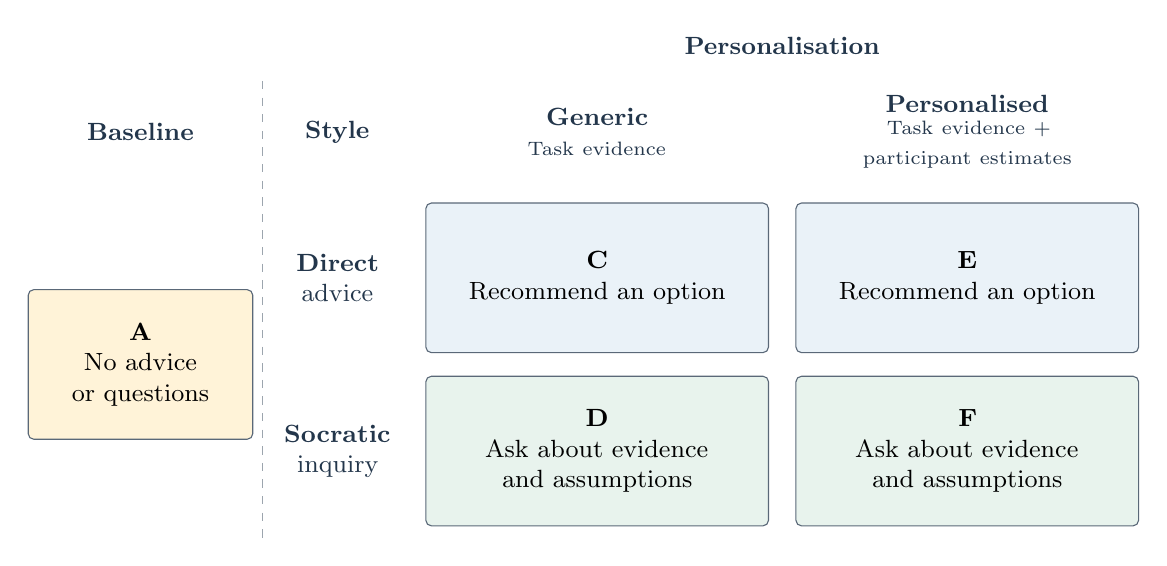
\begin{tikzpicture}[
  condition/.style={box,text width=40mm,minimum height=19mm},
  heading/.style={align=center,font=\small,text=ink},
  columnheading/.style={heading,text width=40mm,minimum height=13mm,anchor=south}
]
\node[heading,font=\small\bfseries] at (1.85,1.85) {Personalisation};
\node[columnheading] at (-.5,.1) {\textbf{Generic}\\{\scriptsize Task evidence}};
\node[columnheading] at (4.2,.1) {\textbf{Personalised}\\{\scriptsize Task evidence +\\participant estimates}};
\node[heading,font=\small\bfseries] at (-3.8,.75) {Style};
\node[heading,text width=17mm] at (-3.8,-1.1) {\textbf{Direct}\\advice};
\node[heading,text width=17mm] at (-3.8,-3.3) {\textbf{Socratic}\\inquiry};
\node[condition] at (-.5,-1.1) {\textbf{C}\\Recommend an option};
\node[condition] at (4.2,-1.1) {\textbf{E}\\Recommend an option};
\node[condition,fill=policygreen] at (-.5,-3.3) {\textbf{D}\\Ask about evidence\\and assumptions};
\node[condition,fill=policygreen] at (4.2,-3.3) {\textbf{F}\\Ask about evidence\\and assumptions};
\node[heading,font=\small\bfseries] at (-6.3,.75) {Baseline};
\node[private,text width=25mm,minimum height=19mm] at (-6.3,-2.2) {\textbf{A}\\No advice\\or questions};
\draw[dashed,draw=ink!45] (-4.75,1.4) -- (-4.75,-4.4);
\end{tikzpicture}
\caption{Five-condition comparison: A provides the no-assistance baseline outside the $2\times2$ matrix, which crosses communication style with personalisation. Generic assistance remains task-aware; personalised assistance additionally uses uncertain participant estimates. All assisted conditions retain uncertainty and objections and may remain silent.}
\label{fig:conditions-matrix}
\end{figure}

Figure~\ref{fig:conditions-matrix} summarises this design. All four assisted conditions retain the distinction between observations and interpretations, preserve relevant objections and permit silence when support is insufficient or interruption is unwarranted. Productive ignorance is therefore a shared design commitment whose expression varies across the conditions; the comparison does not presume that asking questions will prevent premature closure or outperform qualified advice.

Our aim is to make extensive use of the existing empirical evidence to refine the prototype's participant estimates, reasoning rules and intervention policies before conducting a new human assistance study. Repeated simulations with the same reconstructed individuals and fresh outcome realisations will allow us to examine how these design choices interact with different decision-making profiles and task demands. The previous unassisted data constrain the models of task behaviour; responses to assistance remain explicit assumptions to be varied and subsequently tested with people. A methodological contribution is the separation of the synthetic participant, its assumed response to assistance, the assistant's uncertain participant model, graph reasoning and delivery policy, making each component available for inspection and refinement.

\section{Empirical setting and task fidelity}

Our MAB context uses changing reward contingencies, making the interpretation of feedback and the revision of learned expectations central to performance. The full protocol consists of 200 choices among six options, with 50 initially stable trials and 150 volatile trials. Outcome probabilities are hidden. Participants infer values from observed feedback and balance exploration against exploitation. Current prototype options offer gain/zero/loss outcomes at magnitudes of 100 or 200 points; a missed choice incurs a 200-point penalty. Persistence after disappointing feedback can reflect noisy outcomes, a deliberate strategy or a failure to adapt. The observation alone does not distinguish these interpretations.

In our TBS context, two alternatives display their possible gains and win probabilities, but the consequences of a choice depend on progress towards a block target and the contracting horizon. The full protocol consists of 192 choices in 24 eight-trial blocks. A final-trial win multiplies the accumulated block total; a final-trial loss does not activate that multiplier. A missed response consumes an opportunity without a direct point penalty. Immediate expected reward and probability of attaining the target are distinct criteria.

The original tasks use a five-second response limit. The prototype also provides short engineering protocols of 40 MAB trials and 24 TBS trials. These shortened runs support testing and familiarisation; they cannot be substituted for the original protocols when claiming empirical reconstruction fidelity.

\subsection{Empirical cohort and multilevel configurations}
The collaboration draws on an existing experimental programme using two decision environments~\cite{briefing,instructions}. The research materials describe a 62-person cohort with continuous, task-specific profiles combining psychological dispositions, resting-state and task-evoked neural measures, computational measures and behavioural policies. Task performance was examined separately and was excluded from profile scoring and assignment. Four exploratory multilevel configurations describe how the MAB-related and TBS-related profiles are jointly expressed:
\begin{itemize}
  \item \textbf{MAB-specialised.} More pronounced expression of the MAB-related profile, with lower expression of the TBS-related profile. This configuration emphasises the combination of measures associated with decision-making under uncertain and changing reward contingencies.
  \item \textbf{TBS-specialised.} More pronounced expression of the TBS-related profile, with lower expression of the MAB-related profile. This configuration emphasises the combination of measures associated with adjusting decisions to targets, accumulated resources and remaining opportunities.
  \item \textbf{Dual-regime.} Pronounced expression of both task-related profiles. The configuration captures the coexistence of the distinct multilevel patterns associated with the two decision environments, without implying that the same mechanisms support both.
  \item \textbf{Low-expression.} Lower expression of both task-related profiles. This describes the position of an individual on the constructed profile dimensions; it does not by itself establish generally poor decision-making or an absence of relevant abilities.
\end{itemize}
Continuous task-specific scores accompany these descriptions. The configurations are descriptive rather than validated fixed personality types, and neither their neural components nor SFSS dispositional scores establish responsiveness to AI. Some integrated analyses in the briefing use 60 participants; sample availability and exclusions must therefore be reconciled for each reconstruction and validation analysis.

\section{Experimental design: five conditions and staged validation}
\subsection{Factorial comparison and baseline}
The implemented condition set is shown in Table~\ref{tab:conditions}. Generic means \emph{task-aware but non-personalised}. The earlier task-unaware guidance condition has been removed and is not part of this design. Condition letters are retained for continuity with the software.

\begin{table}[H]
\centering\small
\begin{tabularx}{\linewidth}{@{}lYYY@{}}
\toprule
Condition & Communication & Permitted task evidence & Participant calibration \\
\midrule
A & No assistance & Available to the task runner & Withheld from assistance \\
C & Direct recommendation & Current public state and observed history & Withheld \\
E & Direct recommendation & Same task evidence & Used with uncertainty \\
D & Socratic question & Current public state and observed history & Withheld \\
F & Socratic question & Same task evidence & Used with uncertainty \\
\bottomrule
\end{tabularx}
\caption{A no-assistance baseline plus a $2\times2$ comparison of style and personalisation. All conditions complete the required unassisted calibration; only E/F use its participant estimates to select assistance.}
\label{tab:conditions}
\end{table}

For a prespecified outcome $Y$, oriented so that larger values mean improvement, the factorial contrasts within each task are
\begin{align}
\Delta_{\mathrm{style}} &= \tfrac12[(Y_D-Y_C)+(Y_F-Y_E)],\\
\Delta_{\mathrm{person}} &= \tfrac12[(Y_E-Y_C)+(Y_F-Y_D)],\\
\Delta_{\mathrm{interaction}} &= (Y_F-Y_E)-(Y_D-Y_C).
\end{align}
Each assisted condition is also compared with A. These are proposed analytical contrasts, not estimates computed from human data. Task outcomes have different units and will not be pooled by subtracting raw MAB and TBS scores.

\subsection{All 62 as the target; 16 for development}
We propose obtaining the available data and specifications for all 62 participants at the outset. Sixteen individuals, four from each exploratory profile, form an initial development subset. Selection criteria should be agreed before examining assistance outcomes and should cover variation within profiles rather than only high-fitting or especially clear examples. Each agent retains an individual policy for each task; a profile is not a substitute for a generative model.

After developing the data mapping and modelling procedure, we will freeze the procedure and evaluate the remaining 46 participants. Development-subset and remaining-cohort results will be reported separately as well as together. This participant-level separation does not replace holding out trials within an individual for choice prediction. Missing or unusable data may reduce the analysable sample and will be reported rather than silently replaced.

\begin{figure}[tbp]
\centering
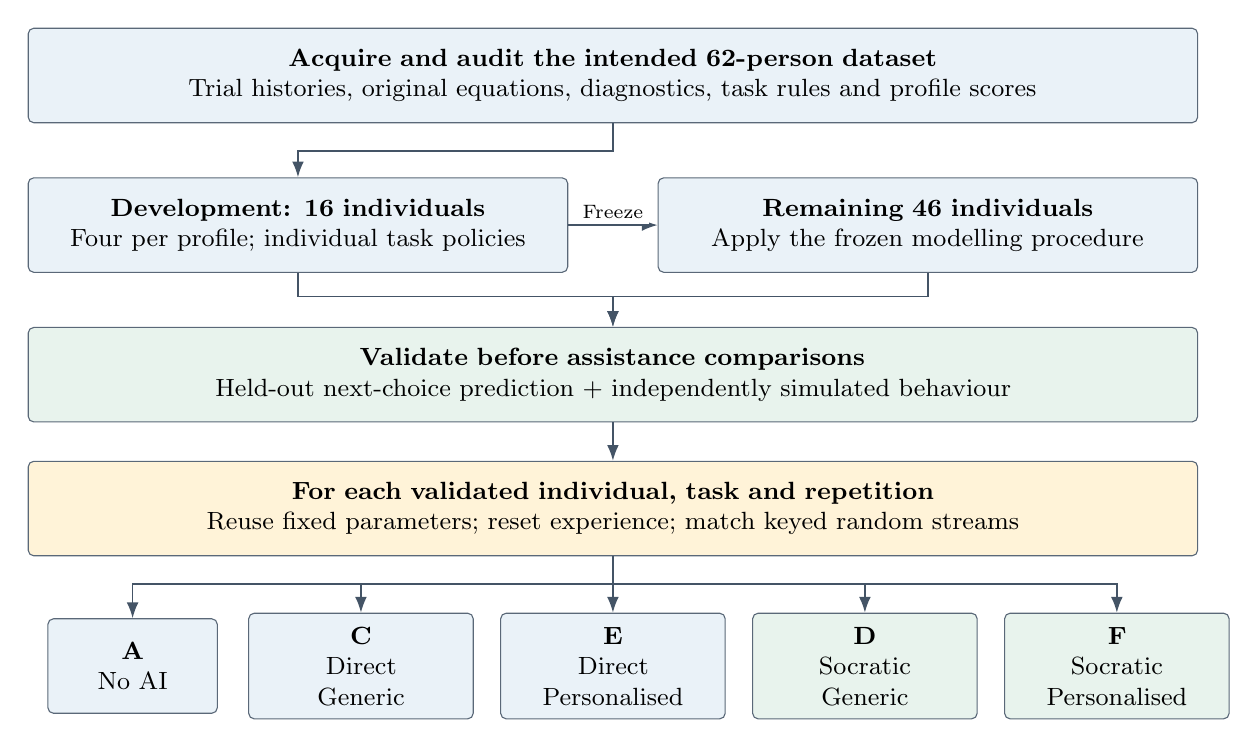
\begin{tikzpicture}
\node[box,text width=145mm] (data) at (0,0)
  {\textbf{Acquire and audit the intended 62-person dataset}\\
   Trial histories, original equations, diagnostics, task rules and profile scores};
\node[box,text width=65mm] (dev) at (-4,-1.9)
  {\textbf{Development: 16 individuals}\\Four per profile; individual task policies};
\node[box,text width=65mm] (remaining) at (4,-1.9)
  {\textbf{Remaining 46 individuals}\\Apply the frozen modelling procedure};
\draw[arrow] (data.south) -- ++(0,-.35) -| (dev.north);
\draw[arrow] (dev.east) -- node[lab,above]{Freeze} (remaining.west);
\node[policy,text width=145mm] (validate) at (0,-3.8)
  {\textbf{Validate before assistance comparisons}\\
   Held-out next-choice prediction $+$ independently simulated behaviour};
\draw[arrow] (dev.south) -- ++(0,-.3) -| (validate.north);
\draw[arrow] (remaining.south) -- ++(0,-.3) -| (validate.north);
\node[private,text width=145mm] (reset) at (0,-5.5)
  {\textbf{For each validated individual, task and repetition}\\
   Reuse fixed parameters; reset experience; match keyed random streams};
\draw[arrow] (validate) -- (reset);
\node[box,text width=18mm] (a) at (-6.1,-7.5) {\textbf{A}\\No AI};
\node[box,text width=25mm] (c) at (-3.2,-7.5) {\textbf{C}\\Direct\\Generic};
\node[box,text width=25mm] (e) at (0,-7.5) {\textbf{E}\\Direct\\Personalised};
\node[policy,text width=25mm] (d) at (3.2,-7.5) {\textbf{D}\\Socratic\\Generic};
\node[policy,text width=25mm] (f) at (6.4,-7.5) {\textbf{F}\\Socratic\\Personalised};
\draw[arrow] (reset.south) -- ++(0,-.35) -| (a.north);
\draw[arrow] (reset.south) -- ++(0,-.35) -| (c.north);
\draw[arrow] (reset.south) -- (e.north);
\draw[arrow] (reset.south) -- ++(0,-.35) -| (d.north);
\draw[arrow] (reset.south) -- ++(0,-.35) -| (f.north);
\end{tikzpicture}
\caption{Proposed empirical development and matched simulation design. Generic conditions remain task-aware. The reset applies to synthetic actors; human participants cannot be assumed to forget previous conditions.}
\label{fig:study}
\end{figure}

\subsection{Two validation problems before assistance effects}
First, in \emph{next-choice prediction}, the model receives the actual information and preceding feedback available to the participant. It predicts a distribution over the next choice. Evaluation will include probabilistic predictive quality and comparison with simple task-appropriate baselines. Parameters fitted using all trials cannot establish held-out predictive accuracy on those same trials. Training and validation splits must respect task chronology, with no future choices entering parameter estimation, preprocessing or model selection.

Second, in \emph{independent simulation}, the agent generates its own choices and updates from its own feedback under fresh outcome realisations. We will examine performance distributions and behavioural adjustment measures, including feedback-conditioned switching and sensitivity to changing constraints. Agreement on a final score alone is insufficient. Parameter recovery and model validation are complementary checks~\cite{wilson}. Their precise implementation, thresholds and reserved measures remain to be agreed before empirical evaluation.

Profile-defining quantities will be distinguished from independent validation outcomes. Otherwise, reproducing a measure used to construct a profile could be mistaken for external validation of that profile. The original equations, parameter definitions, fitting code and diagnostics are needed before importing coefficients into either generative policy, especially TBS.

\subsection{Matched runs, response assumptions and interpretation}
In each synthetic comparison, fixed characteristics persist but experience and the task environment start afresh. Calibration observations are generated or provided separately; the assistant's calibration does not initialise the actor with experience from a previous comparison. A condition-independent keyed random source coordinates choices, environmental changes, option pairs and outcomes. Under zero assistance responsiveness, all conditions must yield identical choices and outcomes for the same individual, task and repetition. When choices diverge, matching the random source does not require identical realised rewards.

Response scenarios currently include null, responsive and interference settings. Both styles use explicit parameters for responsiveness, reactance, distraction and omission. Direct advice supplies an action target; Socratic intervention invokes a task-specific reconsideration heuristic without supplying a recommended option. Reconsideration can retain the original preference. These are assumptions for sensitivity analysis, not response estimates derived from the original unassisted experiment. We will vary parameter uncertainty and response assumptions rather than report one assumed mechanism as a human treatment effect.

The proposed primary task outcomes are MAB total reward and TBS block target attainment, supplemented by behavioural adaptation and interference measures. Weaker-task status must be defined from prespecified baseline evidence rather than assisted outcomes or incomparable raw task scores. Dual-regime and Low-expression profiles need not have a unique weaker environment. Repeated unassisted baselines and appropriate comparisons are needed to address regression to the mean. Replications reduce Monte Carlo uncertainty; they do not create additional independent participants. Cohort-level inference, uncertainty intervals and multiplicity control remain part of the prospective analysis plan.

\section{Architecture: separate epistemic and behavioural responsibilities}
The preceding comparisons require independent control of how a participant acts, what the assistant can observe, which interpretations the evidence supports and whether communicating an interpretation is worthwhile. If these responsibilities are conflated, an apparent assistance benefit could arise from access to hidden task information or an assumed participant response, while a fluent explanation could obscure the uncertainty behind an intervention. The architecture therefore gives productive ignorance a concrete role in the experiment: limitations in evidence constrain the reasons available to the assistant, unresolved objections constrain what it may claim, and interruption costs constrain whether it should speak. Separating these responsibilities also allows participant models, reasoning rules and delivery policies to be refined and evaluated independently.

Figure~\ref{fig:architecture} shows how these separations organise the interaction loop. The upper, gold-coloured components belong to the researcher-side simulation. The private environment generates task states and outcomes; the synthetic participant makes choices using its own task policy, experience and assumed response to assistance; and the evaluator retains the private information needed to interpret performance and paired comparisons. The validated public-event interface below them is the boundary between this machinery and the assistant. It admits permitted task displays, observed choices and outcomes, and attributed participant reports, while withholding hidden reward probabilities, future outcomes and the actor's latent parameters. The condition filter additionally controls the use of participant estimates, so that personalisation in E/F depends on uncertain calibration rather than privileged knowledge of the simulated individual.

\begin{figure}[H]
\centering
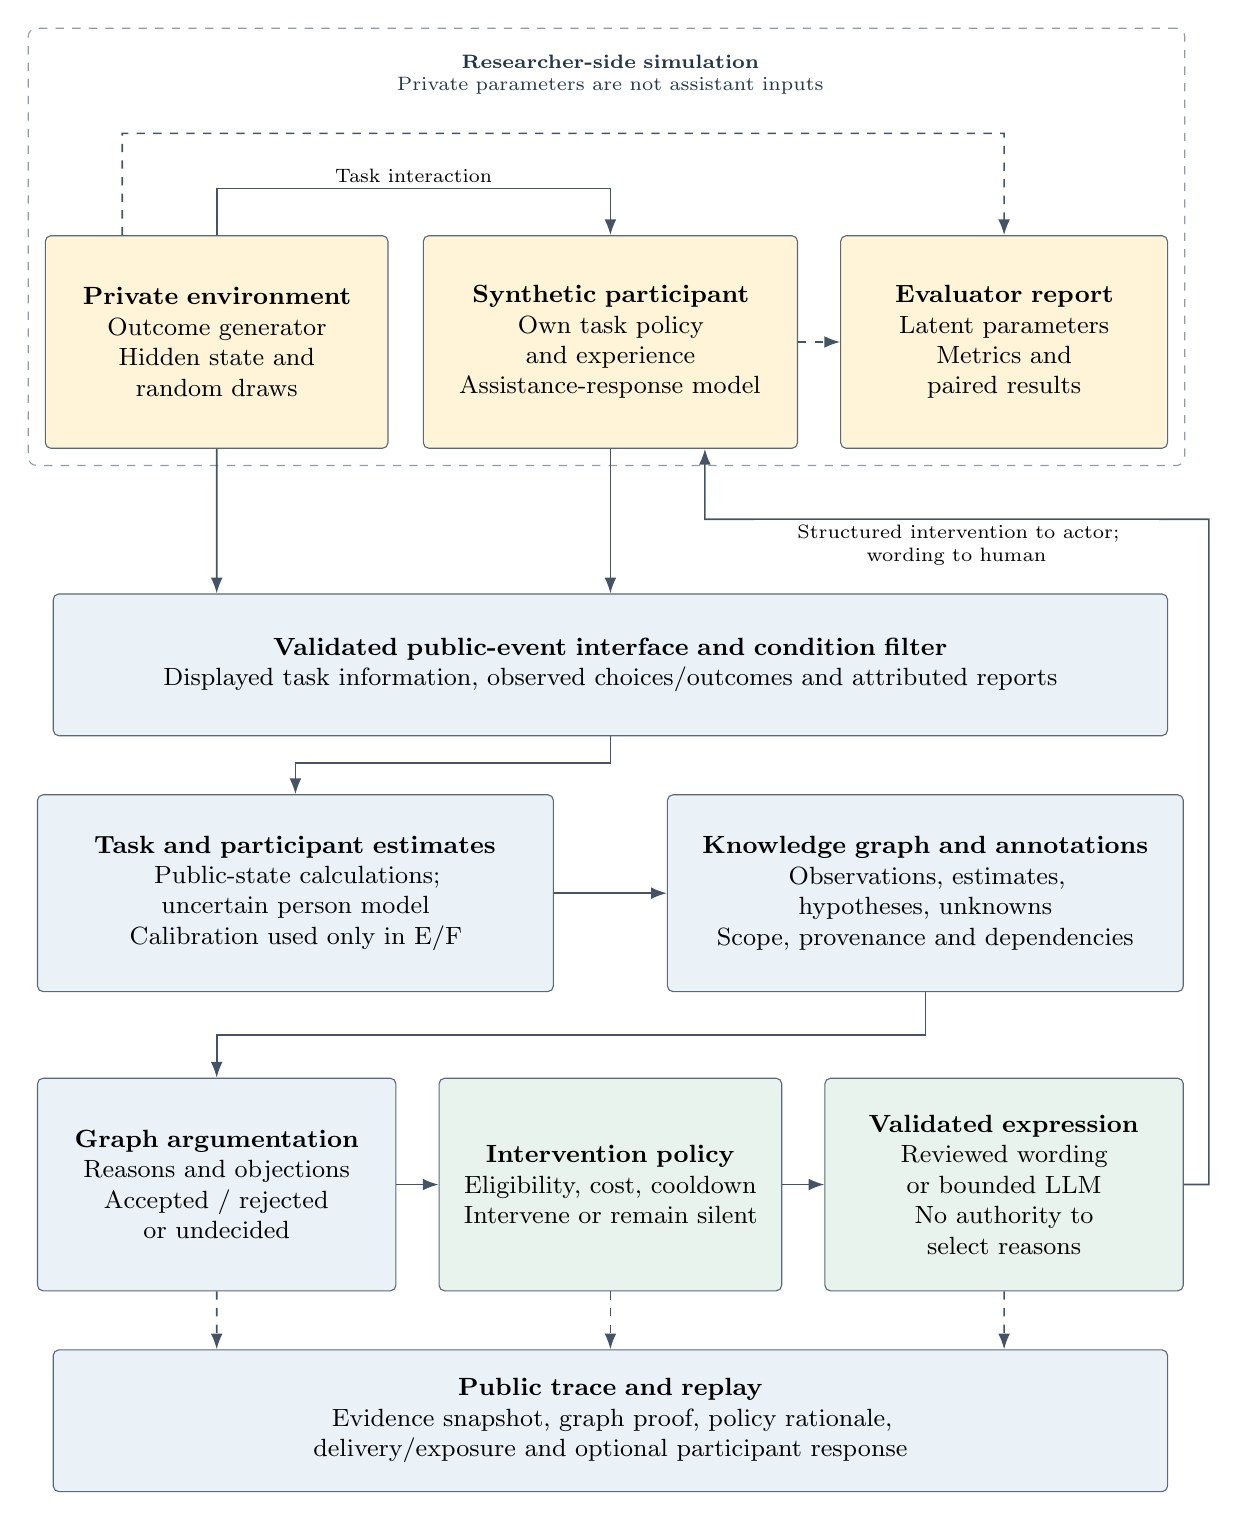
\begin{tikzpicture}[
  architecturetop/.style={private,minimum height=27mm},
  architecturemodel/.style={box,text width=62mm,minimum height=25mm},
  architecturestep/.style={box,minimum height=27mm}
]
% Researcher-side components and separate overhead routing lanes.
\node[architecturetop,text width=40mm] (env) at (-5,0)
  {\textbf{Private environment}\\Outcome generator\\Hidden state and\\random draws};
\node[architecturetop,text width=44mm] (actor) at (0,0)
  {\textbf{Synthetic participant}\\Own task policy\\and experience\\Assistance-response model};
\node[architecturetop,text width=38mm] (eval) at (5,0)
  {\textbf{Evaluator report}\\Latent parameters\\Metrics and\\paired results};
\node[align=center,font=\scriptsize,text=ink,text width=138mm] (simulationtitle) at (0,3.4)
  {\textbf{Researcher-side simulation}\\Private parameters are not assistant inputs};
\draw[arrow] (env.north) -- (-5,1.95)
  -- node[lab,above]{Task interaction} (0,1.95) -- (actor.north);
\draw[recorded] (actor.east) -- (eval.west);
\draw[recorded] ([xshift=-12mm]env.north) -- (-6.2,2.65)
  -- (5,2.65) -- (eval.north);

% Public evidence enters below the simulation; the intervention returns on a separate lane.
\node[box,text width=138mm,minimum height=18mm] (gate) at (0,-4.1)
  {\textbf{Validated public-event interface and condition filter}\\Displayed task information, observed choices/outcomes and attributed reports};
\draw[arrow] (env.south) -- ([xshift=-50mm]gate.north);
\draw[arrow] (actor.south) -- (gate.north);

\node[architecturemodel] (models) at (-4,-7)
  {\textbf{Task and participant estimates}\\Public-state calculations;\\uncertain person model\\Calibration used only in E/F};
\node[architecturemodel] (kb) at (4,-7)
  {\textbf{Knowledge graph and annotations}\\Observations, estimates,\\hypotheses, unknowns\\Scope, provenance and dependencies};
\draw[arrow] (gate.south) -- (0,-5.35) -| (models.north);
\draw[arrow] (models.east) -- (kb.west);

\node[architecturestep,text width=42mm] (graph) at (-5,-10.7)
  {\textbf{Graph argumentation}\\Reasons and objections\\Accepted / rejected\\or undecided};
\node[architecturestep,text width=40mm,fill=policygreen] (policy) at (0,-10.7)
  {\textbf{Intervention policy}\\Eligibility, cost, cooldown\\Intervene or remain silent};
\node[architecturestep,text width=42mm,fill=policygreen] (language) at (5,-10.7)
  {\textbf{Validated expression}\\Reviewed wording\\or bounded LLM\\No authority to\\select reasons};
% This connector stays in the open corridor above all three lower components.
\draw[arrow] (kb.south) -- (4,-8.8) -- (-5,-8.8) -- (graph.north);
\draw[arrow] (graph.east) -- (policy.west);
\draw[arrow] (policy.east) -- (language.west);

\node[box,text width=138mm,minimum height=18mm] (trace) at (0,-13.7)
  {\textbf{Public trace and replay}\\Evidence snapshot, graph proof, policy rationale,\\delivery/exposure and optional participant response};
\draw[recorded] (graph.south) -- ([xshift=-50mm]trace.north);
\draw[recorded] (policy.south) -- (trace.north);
\draw[recorded] (language.south) -- ([xshift=50mm]trace.north);
% The return arrow remains outside the graph and gate and enters a distinct actor port.
\draw[arrow] (language.east) -- (7.6,-10.7) -- (7.6,-2.25)
  -- node[lab,below,text width=50mm]{Structured intervention to actor;\\wording to human} (1.2,-2.25)
  -- ([xshift=12mm]actor.south);
\begin{scope}[on background layer]
\node[frame,fit=(env)(actor)(eval)(simulationtitle)] {};
\end{scope}
\end{tikzpicture}
\caption{Architecture separating participant behaviour, epistemic assessment and intervention delivery. Gold boxes contain private simulation components; the public-event interface restricts the evidence available to the assistant. Below that boundary, numerical models inform an annotated knowledge graph, argumentation evaluates reasons and objections, and a separate policy determines whether and how to intervene. Validated expression returns the intervention to the participant, while the trace retains its evidential and delivery history. Solid arrows show operational flow; dashed arrows show evaluator or trace records.}
\label{fig:architecture}
\end{figure}

Below the information boundary, task calculations and uncertain participant estimates populate the knowledge graph with their provenance, scope and epistemic status. Graph argumentation then constructs supporting reasons and objections and evaluates arguments as accepted, rejected or undecided. This is the epistemic part of the architecture: it determines which grounds for communication survive the current evidence and rules, without turning an accepted model-based inference into an observed fact. The intervention policy performs a different assessment, combining condition eligibility, relevance, interruption cost and recent delivery history. An accepted reason may consequently produce no message, while a permitted unresolved conflict may support a clarification question in D/F. The final expression component renders the selected intervention through reviewed wording or a bounded language-model mode; it has no authority to invent reasons or settle objections.

The return arrow closes the behavioural loop: a synthetic actor receives a structured intervention processed by the separate assistance-response model, whereas a human participant encounters its wording in the task interface. Subsequent choices and optional responses supply new public observations for later assessments. Along the bottom of the figure, the trace records the evidence snapshot, argument evaluation, policy rationale and actual delivery or silence. This makes it possible to distinguish an unsupported interpretation from an unwarranted interruption or a failure to expose the selected message, rather than attributing every outcome to the advice or question alone. In human sessions, the person replaces the synthetic actor while the assistant retains the public-event interface and reasoning pipeline; the simulated response mechanism does not become a model of how that person understands the message.

\subsection{Actor, assistance response and assistant model}
The synthetic actor has its own task parameters and history. The current MAB actor uses dual learning rates with softmax choice. The current TBS actor is a provisional logistic policy over normalised target pressure and has no learned internal state. It is not a reconstruction of the original TBS mechanisms. Environment-specific adapters can replace these policies with models compatible with the empirical data without rewriting the shared experiment runner.

The assistance-response model modifies the actor's choice distribution only when an intervention is delivered. It is distinct from the assistant's participant model. The latter contains estimates from unassisted calibration and permitted observations, not the actor's true learning rates or responsiveness parameters. Giving those latent parameters to personalised assistance would confer an unrealistic information advantage.

Interaction estimates are intentionally narrow. Explicit reports can describe burden and can adjust interruption cost in E/F. Agreement with a delivered direct recommendation is recorded as concordance, not measured trust, causal compliance or benefit. Socratic reconsideration remains unknown without a report. A disagreement can contest an interpretation without establishing a general aversion to assistance. Personalisation influences intervention selection through participant evidence, without presuming that personalised support is more useful.

\subsection{Knowledge representation and graph reasoning}
\label{sec:knowledge-reasoning}
The knowledge representation connects a proposed intervention to the task state, observations, calculations and assumptions on which it depends. Three complementary elements support this connection:
\begin{itemize}
  \item \textbf{Persistent records.} Canonical JSON events and snapshots are persisted locally in SQLite, including numerical model outputs and delivery-policy records.
  \item \textbf{Graph projection.} A deterministic projection exposes selected records as an RDF graph of subject--predicate--object triples with identifiable resources and typed values~\cite{rdf}.
  \item \textbf{Shared and task-specific vocabularies.} RDF/OWL vocabularies organise a shared epistemic core, a task-independent layer and separate \texttt{mab:} and \texttt{tbs:} namespaces; an \texttt{arg:} extension represents propositions, arguments and attacks.
\end{itemize}
The vocabularies specify the kinds of knowledge the prototype can represent. They do not constitute an unrestricted OWL inference engine: numerical inference runs in Python, while the graph reasoner executes explicitly authored argument schemes.

\subsubsection{Represented knowledge and epistemic status}
Table~\ref{tab:knowledge} how each category of knowledge is encoded and linked to its context and provenance:

\begin{table}[H]
\centering\small
\begin{tabularx}{\linewidth}{@{}>{\raggedright\arraybackslash}p{27mm}Y>{\raggedright\arraybackslash}p{39mm}@{}}
\toprule
\textbf{Knowledge} & \textbf{Graph representation} & \textbf{Context and provenance} \\
\midrule
\textbf{Mechanics and state} & \texttt{task:TaskDefinition}, \texttt{task:Rule}, \texttt{task:Option} and \texttt{task:TaskState}; domain properties describe arms, gambles, points, targets and horizon. & Task version, trial, phase and previous state. \\
\midrule[0.3pt]
\textbf{Observations} & \texttt{task:ChoiceObservation} and \texttt{task:OutcomeObservation}; selected option, reward, timeout and response time. & Source trial and the choice to which an outcome belongs. \\
\midrule[0.3pt]
\textbf{Calculations and estimates} & \texttt{task:Calculation} and \texttt{task:Estimate}; typed values, units, sample counts and available uncertainty bounds. & Input state, named versioned rule, option and supporting observations. \\
\midrule[0.3pt]
\textbf{Claims and reports} & Core claims and hypotheses, plus \texttt{arg:Assertion} records with scoped propositions and attributed participant reports. & Source, epistemic status, dependencies, contestation and revision links where applicable. \\
\midrule[0.3pt]
\textbf{Arguments and attacks} & \texttt{arg:Argument} and \texttt{arg:Attack}; premises, conclusion, subarguments, scheme, attack target and evaluation label. & Rule identity, inference kind, priority and links to the intervention or considered objection. \\
\bottomrule
\end{tabularx}
\caption{Knowledge represented in the assistant-side graph. Numerical models compute values before projection; the graph preserves their meaning and provenance. Candidate scores, interruption costs and cooldowns remain in the canonical JSON policy records.}
\label{tab:knowledge}
\end{table}

\begin{itemize}
  \item \textbf{Mechanics and state.} Public task definitions and current decision contexts include MAB arms, displayed TBS gambles, targets and conditional scoring rules. Dynamic states identify the trial and phase and describe quantities such as accumulated points, target gap and remaining choices.
  \item \textbf{Observations.} Records of selected options, received rewards, timeouts and response times describe what occurred in the task. Choices and outcomes are represented separately and remain distinguishable from calculations or interpretations based on them.
  \item \textbf{Calculations and estimates.} Derived quantities include MAB sampled-arm counts, reward beliefs, change estimates and learned values, as well as TBS expected gains and final-choice attainment probabilities. Estimates of the participant's task policy also belong here and retain their evidence and uncertainty.
  \item \textbf{Claims and reports.} Claims express task interpretations and provisional behavioural hypotheses based on the available evidence. Attributed participant reports can supply a stated strategy or contest an interpretation; their source and epistemic status distinguish them from observations and model outputs.
  \item \textbf{Arguments and attacks.} Explicit reasoning records connect premises to conclusions through named schemes and retain objections to premises, conclusions or rule applicability. Their evaluation labels show which grounds for communication are accepted, rejected or unresolved.
\end{itemize}
Hidden MAB probabilities, realised change times and future outcomes remain outside this assistant-side representation.



A derived quantity links to its input state through \texttt{task:inputState}, to the calculation rule through \texttt{task:usesRule}, and, where relevant, to an option or supporting observation. Thus a reward estimate can be traced to sampled outcomes, while displayed-input arithmetic can be traced to the current option and published scoring rule. Claims carry epistemic annotations such as known, unknown, assumed, inferred, contested, probable, low-confidence and source-dependent; these need not be mutually exclusive. Relations including \texttt{supportedBy}, \texttt{dependsOn}, \texttt{contradicts} and \texttt{revises} retain evidential and revision history. Unknown is not interpreted as false, and a participant's disagreement is recorded as an attributed report rather than silently replacing an observation or numerical posterior.

For reasoning, an \texttt{arg:Assertion} wraps a structured proposition $\langle s,p,o,\sigma,\epsilon\rangle$: subject, predicate, typed object, current-state scope and positive or negative polarity. The assertion separately records its kind, source and epistemic statuses. For example, a TBS state's \texttt{tbs:points} value can be a known observation, whereas a pressure-sensitivity estimate is inferred and source-dependent. Accepting an argument that uses the latter does not establish an observed disposition. Explicit scope also prevents a comparison made before a choice from being attributed to the state after its outcome.

\subsubsection{Argument construction and evaluation}
The implementation separates model calculation, argument discovery and argument evaluation. Python computes Bayesian reward estimates and task arithmetic; an optional pgmpy backend supports a small interpretation network with authored probability tables. These numerical outputs supply premises, not argument priorities or diagnoses. The graph pipeline then proceeds as follows:
\begin{enumerate}
  \item \textbf{Project the current evidence.} The reasoner builds a local graph from the current task snapshot, permitted history aggregates, eligible model hypotheses and scoped participant reports. Numeric state, option, goal and calculation records become explicit assertions. Re-analysis of an earlier event uses only its recorded history prefix, excluding later feedback or reviews.
  \item \textbf{Instantiate authored schemes.} Locally versioned SPARQL \texttt{SELECT} queries~\cite{sparql} run through RDFLib to find premises satisfying a scheme's graph patterns and numerical conditions. Each match must return existing assertion identifiers from the same state. It creates an argument recording its premises, conclusion, subarguments, rule identity and strict or defeasible inference kind. Derived assertions can support further schemes in bounded forward rounds; circular self-support is excluded. Queries cannot execute updates or remote services, and participant or language-model text does not become an executable rule.
  \item \textbf{Construct attacks and defeats.} An argument can undermine a contrary estimated, reported or assumed premise, rebut a contrary defeasible conclusion, or undercut the applicability of a named defeasible scheme. Contrariness requires explicit opposite polarities over the same scoped proposition; missing evidence and different decision criteria do not count as contradictions. Successful attacks propagate to arguments containing the defeated subargument. Authored priorities govern rebuttal and undermining; undercutting is independent of those priorities. The initial schemes use equal priorities, independently of Bayesian confidence and intervention usefulness.
  \item \textbf{Compute grounded labels.} A finite fixed-point procedure accepts an argument when all its defeaters are rejected, rejects it when a defeater is accepted, and leaves unresolved dependencies or cycles undecided~\cite{dung}. The epistemic status known is assigned only to strict conclusions with exclusively known premises; other derived conclusions remain inferred. Argument labels express justification under the recorded premises and rules, rather than truth or measured usefulness. The subsequent policy can select only condition-permitted, proof-backed communication opportunities.
\end{enumerate}

Python validates schemas, arithmetic, proof links, acyclicity and state consistency. When pySHACL is installed, SHACL additionally checks constraints on the RDF projection~\cite{shacl}; this checks structural conformance rather than empirical truth. Current discovery limits are six rounds, 256 arguments, 512 assertions and 1,024 query matches per snapshot. Reaching a construction limit marks the analysis incomplete and all argument labels undecided, because an undiscovered objection might change an apparent acceptance; the delivery policy then remains silent. Unavailable RDF reasoning likewise produces no intervention. Fixed rule order, sorted matches, content-derived identifiers and frozen configuration hashes support replay. These bounds and checks constrain execution without establishing real-time performance or scientific validity.

\subsubsection{Two illustrative reasoning traces}
The implemented example runner generated these synthetic traces in unassisted calibration, where condition A remains silent. Their possible use in assisted conditions is subject to the separate delivery policy.

\paragraph{MAB: limited coverage does not settle the value of exploration.} After seven observed choices have sampled only one of six arms, a strict coverage scheme derives that alternatives remain unsampled. A defeasible scheme then concludes that further exploration is worth discussing; it does not conclude that the participant has made an error. In a later snapshot with only two choices remaining, a second defeasible scheme uses the short horizon to oppose that same conclusion. With equal priorities, both exploration arguments remain undecided, while the arithmetic coverage conclusion remains accepted. A separate short-horizon undercutter blocks a personalised challenge based on underexploration. In D/F, an explicitly authored clarification may nevertheless ask, ``With so few decisions remaining, what would you gain from trying another option?'' C/E cannot derive advice from the undecided exploration warrant, although unrelated accepted reasons remain available. Productive ignorance here preserves both the information gap and the objection to acting on it.

\paragraph{TBS: compatible calculations can favour different choices.} Before the final choice, suppose the accumulated total is 200 points, the target is 930 and the multiplier is 2.3. The displayed alternatives offer a gain of 180 with probability 0.60 and a gain of 260 with probability 0.35. Python computes immediate expected gains and totals conditional on a final win:
\begin{align*}
\mathrm{EV}_{\mathrm{safe}} &= 0.60\times180=108,
& \mathrm{EV}_{\mathrm{risky}} &= 0.35\times260=91,\\
W_{\mathrm{safe}} &= (200+180)\times2.3=874,
& W_{\mathrm{risky}} &= (200+260)\times2.3=1058.
\end{align*}
The final-choice attainment probabilities are therefore zero and 0.35, respectively: a loss leaves 200 points and does not activate the multiplier. The graph stores expected-gain and attainment calculations as distinct typed resources, each linked to the input state, option and rule, with units of points or probability. Strict schemes establish the two rankings and then derive \texttt{tbs:criteriaDiverge}. These conclusions are compatible because they concern different criteria. A further defeasible scheme supports clarifying the objective, without claiming to know the participant's intention. Its reviewed Socratic wording asks, ``Expected gain and final target attainment favour different options. Which objective guides your choice?'' C/E require an additional accepted option-comparison proof to recommend an action under their stated criterion. The trace thus exposes how a mathematically correct calculation can support a question about the grounds for choosing, rather than manufacture a single unconditional answer.

\subsection{From justified reasons to justified interruption}
Graph argumentation is the single source of live reasons and objections. The policy selects among graph-grounded communication opportunities; it cannot invent a separate reason when graph reasoning fails. Supported content and a useful interruption remain different questions (Figure~\ref{fig:policy}). Usefulness, interruption cost, thresholds and cooldowns are explicit, provisional policy parameters. The policy does not establish the acceptance of an argument.

\begin{figure}[H]
\centering
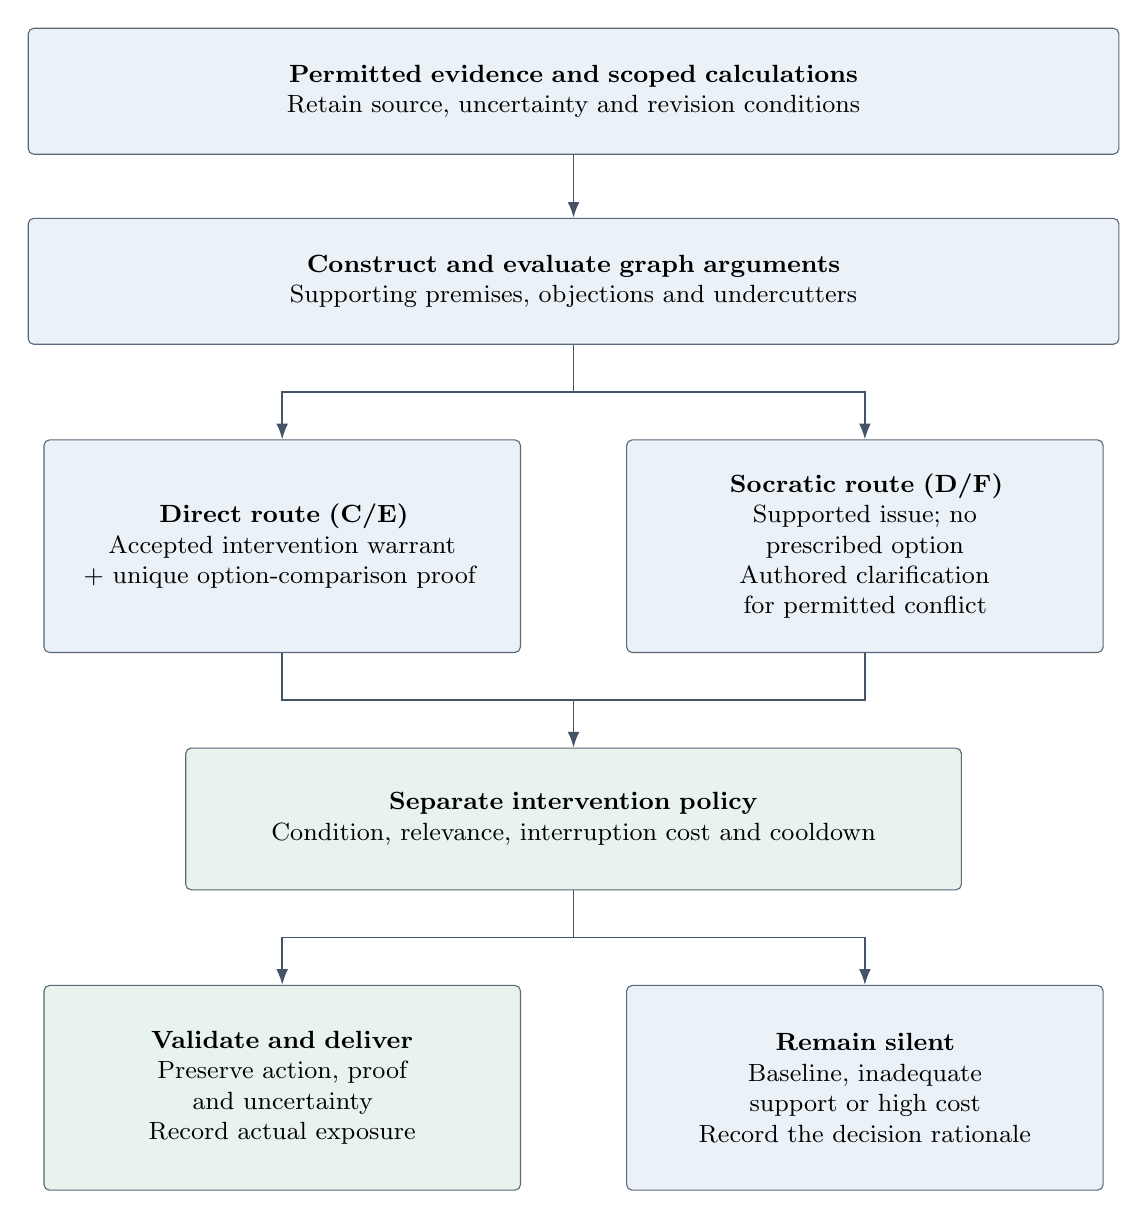
\begin{tikzpicture}[
  policywide/.style={box,text width=135mm,minimum height=16mm},
  policyroute/.style={box,text width=57mm,minimum height=27mm},
  policyoutcome/.style={box,text width=57mm,minimum height=26mm},
  connector/.style={semithick,draw=ink!85}
]
\node[policywide] (input) at (0,0)
  {\textbf{Permitted evidence and scoped calculations}\\Retain source, uncertainty and revision conditions};
\node[policywide,below=8mm of input] (proof)
  {\textbf{Construct and evaluate graph arguments}\\Supporting premises, objections and undercutters};
\draw[arrow] (input.south) -- (proof.north);

% Common-height routes leave an open branching corridor above both boxes.
\coordinate (routebranch) at ($(proof.south)+(0,-6mm)$);
\node[policyroute,anchor=north] (direct) at ($(routebranch)+(-37mm,-6mm)$)
  {\textbf{Direct route (C/E)}\\Accepted intervention warrant\\$+$ unique option-comparison proof};
\node[policyroute,anchor=north] (socratic) at ($(routebranch)+(37mm,-6mm)$)
  {\textbf{Socratic route (D/F)}\\Supported issue; no\\prescribed option\\Authored clarification\\for permitted conflict};
\draw[connector] (proof.south) -- (routebranch);
\draw[arrow] (routebranch) -| (direct.north);
\draw[arrow] (routebranch) -| (socratic.north);

% Merge below both routes before entering the policy through a single arrow.
\coordinate (routemerge) at ($(direct.south)!0.5!(socratic.south)+(0,-6mm)$);
\node[policy,text width=95mm,minimum height=18mm,anchor=north] (select) at ($(routemerge)+(0,-6mm)$)
  {\textbf{Separate intervention policy}\\Condition, relevance, interruption cost and cooldown};
\draw[connector] (direct.south) |- (routemerge);
\draw[connector] (socratic.south) |- (routemerge);
\draw[arrow] (routemerge) -- (select.north);

% Both outcomes begin below a separate, unobstructed branching corridor.
\coordinate (deliverybranch) at ($(select.south)+(0,-6mm)$);
\node[policyoutcome,fill=policygreen,anchor=north] (deliver) at ($(deliverybranch)+(-37mm,-6mm)$)
  {\textbf{Validate and deliver}\\Preserve action, proof\\and uncertainty\\Record actual exposure};
\node[policyoutcome,anchor=north] (silent) at ($(deliverybranch)+(37mm,-6mm)$)
  {\textbf{Remain silent}\\Baseline, inadequate\\support or high cost\\Record the decision rationale};
\draw[connector] (select.south) -- (deliverybranch);
\draw[arrow] (deliverybranch) -| (deliver.north);
\draw[arrow] (deliverybranch) -| (silent.north);
\end{tikzpicture}
\caption{Acceptance of an argument does not compel an intervention. Direct advice requires a separate comparison proof. Socratic clarification of unresolved conflict is permitted only by an explicit authored scheme. Incomplete or unavailable reasoning produces no live intervention candidate.}
\label{fig:policy}
\end{figure}

Direct assistance identifies an available option, response key and criterion. MAB compares posterior mean rewards estimated from observed outcomes; this is not an optimal exploration policy. TBS compares immediate expected gains before the final trial and exact one-step target-attainment probability on the final trial, including the conditional multiplier. A strict comparison requires a unique winner. These criteria do not solve multi-trial planning over unknown future options. Socratic interventions instead invite examination of supported issues or uncertainty. A question has no structured recommended option, although its possible indirect steering remains an empirical concern.

Reviewed templates express the selected intervention by default. An experimental local Ollama mode can compose bounded questions for D/F; C/E retain reviewed direct wording. Language packages contain the selected proof closure and actual attackers, not the whole researcher graph. Validation checks grounding and output structure before delivery. Model provider, model version and language mode must be fixed or treated as explicit factors in an empirical experiment. The model does not select graph labels, intervention policy or task actions.

\subsection{Timing, exposure and participant contestation}
The browser interface currently inserts a four-second preparation window in all conditions, including A, followed by the five-second choice window. Delivered messages remain visible through the trial and are dimmed as previous messages afterwards. Optional reply and feedback controls remain visible but accept new responses only for an active intervention in the current trial. Replies do not pause task timers and do not receive an automatic conversational answer. The trace records latency, actual exposure and early choice attempts.

The current TBS backend receives the upcoming option pair during preparation, while the participant sees progress and target information until choices open. This timing is not equivalent to simultaneous information availability. Before a human experiment, exposure must be reconciled so that an intervention does not require a participant to assess an alternative not yet visible. Labels describing intervention eligibility must also match actual screen exposure. Equal nominal windows do not guarantee equal reading opportunities; realised exposure and delivered intervention counts must be reported.

\subsection{Extensibility and reproducibility}
Each registered environment owns event validation, mechanics, numerical models, ontology documents, argument schemes, recommendation wording, actor policy, private simulator, metric definitions and browser adapter. A study JSON selects environments, per-environment protocols, calibration dependencies and conditions. Adding an environment requires its module and assets, registration and study configuration rather than new branches in the shared engine or policy. Metrics declare units and whether to maximise or minimise a quantity.

A third, four-trial REFERENCE environment exercises this contract with its own namespace and an error metric to minimise. It is an engineering fixture, not an additional empirical decision task. Implemented checks cover all five conditions, actor resets, matched null-response behaviour, public/private separation, graph provenance, task completion and replay. Scripted interface checks use actual task scripts with Python persistence; they are not visual or laboratory timing validation. No human assistance effect follows from passing these checks.

Session configurations freeze task, ontology, graph, model and policy descriptors as applicable. Separate evaluator reports retain private specifications, response assumptions, realised choice probabilities, metrics and paired differences. Execution-adapter source fingerprints support drift detection; reproducing a simulation still requires the corresponding code and evaluator inputs. Replay of public events and assistant decisions is distinct from reproducing latent actor choices.

\section{Human implications for national security and governance}
The controlled tasks isolate uncertainty and changing constraints, but omit institutional authority, contested objectives, strategic adversaries and the distribution of harms. We therefore offer design questions for later professional studies, not claims of operational readiness.

\textbf{Intervention authority.} A justified proposition is not automatically a justified interruption. In professional settings, the policy will also need mandate, role and escalation constraints. A logged usefulness score cannot authorise a system to determine public objectives or operational priorities.

\textbf{Contestability and accountability.} Provenance and retained objections can make a particular intervention examinable. Optional disagreement and correction support contestation at the interface. Institutional accountability additionally requires identified decision rights, review procedures and responsibility for model and policy revisions; logs alone do not supply them.

\textbf{Personalisation and agency.} A participant model can expose blind spots, but can also stereotype an individual or tailor persuasive pressure. Keeping estimates uncertain, task-specific and separate from latent parameters is one constraint. Whether this preserves agency must be evaluated with people, rather than inferred from interface labels or recommendation concordance.

\textbf{Preserving uncertainty under pressure.} Productive ignorance does not require endless deliberation. Time-critical work may favour concise qualified advice, escalation or silence. The research question is whether the system helps a person recognise which uncertainties matter within available time, while retaining alternatives for later review.

A subsequent human study will require consent and appropriate review, data minimisation, prespecified endpoints, sample-size planning and random allocation or a justified counterbalanced design. Synthetic resets cannot remove human carryover learning. Workload, comprehension, reasoning quality and appropriate reliance will require measures beyond the current synthetic score reports. Transfer should proceed through expert-designed scenarios with domain-specific goals and evidence rules, followed by independent evaluation.

\section{Current limits and next research steps}
The software provides an inspectable intervention pipeline and a matched simulation framework. It does not yet reconstruct the original cohort. Empirical task-model compatibility, held-out prediction, parameter recovery and independent behavioural validation remain to be completed. Current interpretation probabilities, argument schemes, thresholds and assistance-response mechanisms are authored assumptions. Structural validation and replay constrain software behaviour, not scientific validity.

Synthetic response times and reading exposures are currently placeholders rather than validated models of human timing or workload. Synthetic actors process structured interventions, not natural-language meaning. Any observed difference between assistance styles in these simulations will therefore depend on the chosen response and reconsideration mechanisms.

The next milestone is to obtain and audit the offered data and equations, develop the 16-person reconstruction subset, and evaluate a frozen procedure on the remaining available participants. Only after unassisted fidelity is adequate should assistance comparisons be interpreted, and initially only conditionally on the stated response assumptions. The eventual paper should add the agreed protocol, model and data provenance, empirical validation results, uncertainty analyses and a justified account of relevance beyond the controlled tasks.

\begin{thebibliography}{99}
\bibitem{stanford}
Stanford Center for International Security and Cooperation. \emph{The Future of Decision-Making Project}. Project overview and research goals. \url{https://cisac.fsi.stanford.edu/gtg/future-decision-making}.

\bibitem{daw}
Nathaniel D. Daw, John P. O'Doherty, Peter Dayan, Ben Seymour, and Raymond J. Dolan. Cortical substrates for exploratory decisions in humans. \emph{Nature}, 441:876--879, 2006. \url{https://doi.org/10.1038/nature04766}.

\bibitem{kolling}
Nils Kolling, Marco Wittmann, and Matthew F. S. Rushworth. Multiple neural mechanisms of decision making and their competition under changing risk pressure. \emph{Neuron}, 81(5):1190--1202, 2014. \url{https://doi.org/10.1016/j.neuron.2014.01.033}.

\bibitem{essay}
\emph{The Sophist Machine Needs Productive Ignorance}. Unpublished project essay, undated. Source manuscript retained in the project documentation; publication and authorship details to be confirmed for submission.

\bibitem{briefing}
Irena Danilovska. \emph{Decision-Making Under Uncertainty and Changing Constraints: Empirical Research Briefing for Adaptive AI Decision Support}. Internal research briefing, October 2026. Describes existing studies, not results of the proposed AI-assistance experiment.

\bibitem{instructions}
\emph{Original experimental instructions and task-design clarifications}. Internal collaboration document, undated. Source file: \texttt{original\_experiment\_design.docx}.

\bibitem{bucinca}
Zana Bu\c{c}inca, Maja Barbara Malaya, and Krzysztof Z. Gajos. To Trust or to Think: Cognitive Forcing Functions Can Reduce Overreliance on AI in AI-assisted Decision-making. \emph{Proceedings of the ACM on Human-Computer Interaction}, 5(CSCW1), Article 188, 2021. \url{https://doi.org/10.1145/3449287}.

\bibitem{wilson}
Robert C. Wilson and Anne G. E. Collins. Ten simple rules for the computational modeling of behavioral data. \emph{eLife}, 8:e49547, 2019. \url{https://doi.org/10.7554/eLife.49547}.

\bibitem{shacl}
Holger Knublauch and Dimitris Kontokostas, editors. \emph{Shapes Constraint Language (SHACL)}. W3C Recommendation, 20 July 2017. \url{https://www.w3.org/TR/shacl/}.

\bibitem{rdf}
W3C RDF Working Group. \emph{RDF 1.1 Concepts and Abstract Syntax}. W3C Recommendation, 25 February 2014. \url{https://www.w3.org/TR/rdf11-concepts/}.

\bibitem{sparql}
Steve Harris and Andy Seaborne, editors. \emph{SPARQL 1.1 Query Language}. W3C Recommendation, 21 March 2013. \url{https://www.w3.org/TR/sparql11-query/}.

\bibitem{dung}
Phan Minh Dung. On the acceptability of arguments and its fundamental role in nonmonotonic reasoning, logic programming and n-person games. \emph{Artificial Intelligence}, 77(2):321--357, 1995. \url{https://doi.org/10.1016/0004-3702(94)00041-X}.
\end{thebibliography}
\end{document}
